% Axis E: BAE* / A* expansion ratio as the heuristic weakens.
% Values are exactly those of Table~\ref{tab:xover}; do not edit one without the other.
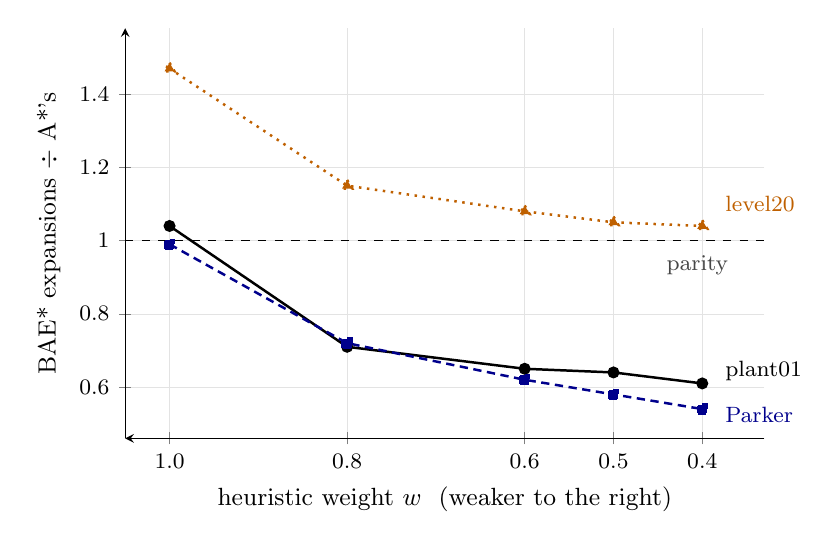
\begin{tikzpicture}
\begin{axis}[
  width=0.80\columnwidth, height=0.56\columnwidth,
  axis lines=left,
  xmin=0.33, xmax=1.05,
  ymin=0.46, ymax=1.58,
  x dir=reverse,
  xtick={1.0,0.8,0.6,0.5,0.4},
  xticklabels={$1.0$,$0.8$,$0.6$,$0.5$,$0.4$},
  ytick={0.6,0.8,1.0,1.2,1.4},
  xlabel={heuristic weight $w$ \ (weaker to the right)},
  ylabel={BAE* expansions $\div$ A*'s},
  label style={font=\small},
  tick label style={font=\footnotesize},
  grid=major,
  grid style={line width=.2pt, draw=gray!22},
  clip=false,
]
% parity: below this line BAE* expands fewer nodes than A*
\addplot[black, dashed, line width=.6pt] coordinates {(1.05,1.0) (0.33,1.0)};
\node[font=\footnotesize, gray!55!black, anchor=north east] at (axis cs:0.36,0.985) {parity};

\addplot[mark=triangle*, mark size=2.1pt, line width=.9pt, color=orange!75!black, dotted]
  coordinates {(1.0,1.47) (0.8,1.15) (0.6,1.08) (0.5,1.05) (0.4,1.04)};
\node[font=\footnotesize, color=orange!75!black, anchor=west] at (axis cs:0.385,1.10) {level20};

\addplot[mark=*, mark size=1.7pt, line width=.9pt, color=black]
  coordinates {(1.0,1.04) (0.8,0.71) (0.6,0.65) (0.5,0.64) (0.4,0.61)};
\node[font=\footnotesize, anchor=west] at (axis cs:0.385,0.645) {plant01};

\addplot[mark=square*, mark size=1.6pt, line width=.9pt, color=blue!55!black, densely dashed]
  coordinates {(1.0,0.99) (0.8,0.72) (0.6,0.62) (0.5,0.58) (0.4,0.54)};
\node[font=\footnotesize, color=blue!55!black, anchor=west] at (axis cs:0.385,0.525) {Parker};
\end{axis}
\end{tikzpicture}
